\subsubsection{bringit::client::view::list::delete::DeleteListView}

\label{bringit::client::view::list::delete::DeleteListView}
\begin{figure}[H]
	\centering
	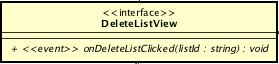
\includegraphics[scale=0.5]{Sezioni/SottosezioniST/img/app/DeleteListView.png}
	\caption{bringit::client::view::list::delete::DeleteListView}
\end{figure}

\begin{itemize}
\item \textbf{Descrizione}: La view relativa alla parte grafica di eliminazione di una lista.
\item \textbf{Utilizzo}: L'interfaccia viene utilizzata per disaccoppiare presenter e implementazione della classe e per visualizzare i dati che gli vengono passati dal presenter.
\item \textbf{Attributi}: 
\item \textbf{Metodi}:
	\begin{itemize}
	\item \textit{public openDeleteListView():void}\\
	Questo metodo mostra il popup relativo all'eliminazione della lista.
	\end{itemize}
\end{itemize} 

\subsubsection{bringit::client::view::list::delete::view::DeleteListViewImpl}

\label{bringit::client::view::list::delete::view::DeleteListViewImpl}
\begin{figure}[H]
	\centering
	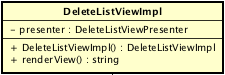
\includegraphics[scale=0.5]{Sezioni/SottosezioniST/img/app/DeleteListViewImpl.png}
	\caption{bringit::client::view::list::delete::view::DeleteListViewImpl}
\end{figure}

\begin{itemize}
\item \textbf{Descrizione}: Questa classe rappresenta la classe concreta di eliminazione di una lista.
\item \textbf{Utilizzo}: Implementando i metodi di DeleteListView questa classe viene utilizzata al momento dell'eliminazione di una lista bringit da Rocket.Chat.
\item \textbf{Attributi}: 
\begin{itemize}
	\item \textit{private presenter:DeleteListViewPresenter}\\
	Il presenter relativo all'eliminazione della lista.
	\item \textit{private deleteEvent:DeleteEventEmitter}\\
	Il riferimento all'oggetto responsabile dell'emissione degli eventi di eliminazione.
	\item \textit{private popup:ShowPopupUseCase}\\
	Il riferimento all'oggetto necessario per il display di popup in Rocket.Chat.
\end{itemize}
\item \textbf{Metodi}:
	\begin{itemize}
	\item \textit{public DeleteListViewImpl():DeleteListViewImpl}\\
	Il costruttore di DeleteListViewImpl.
	\item \textit{public getDeleteEvent():DeleteEventEmitter}\\
	Questo metodo ritorna l'emittitore di eventi di eliminazione utilizzato dalla classe.
	\item \textit{public openDeleteListView(listId:string,nameList:string):void}\\
	Questo metodo mostra il popup relativo all'eliminazione della lista.
					\\ \textbf{Parametri}: \begin{itemize}
			\item \textit{listId:string}\\
			L'identificativo della lista che si vuole eliminare tramite la DeleteListView.
			\item \textit{listId:string}\\
			Il nome della lista che si vuole eliminare.
					\end{itemize} 
	\end{itemize}
\end{itemize} 

\subsubsection{bringit::client::view::list::delete::presenter::DeleteListViewPresenter}

\label{bringit::client::view::list::delete::DeleteListViewPresenter}
\begin{figure}[H]
	\centering
	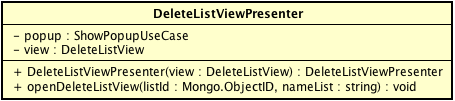
\includegraphics[scale=0.5]{Sezioni/SottosezioniST/img/app/DeleteListViewPresenter.png}
	\caption{bringit::client::view::list::delete::presenter::DeleteListViewPresenter}
\end{figure}

\begin{itemize}
\item \textbf{Descrizione}: Questa classe rappresenta il presenter per la classe di eliminazione della lista bringit.
\item \textbf{Utilizzo}: Il presenter fa da tramite tra l'implementazione e la view, formattando i dati che verranno visualizzati nella view e manipolando gli input dell'utente per eseguire le operazioni logiche predisposte.
\item \textbf{Attributi}: 
	\begin{itemize}
	\item \textit{private groups:string[]}\\
	Array che specifica la posizione del bottone di creazione della lista (ovvero canali, gruppi e messaggi diretti).
	\item \textit{private view:DeleteItemView}\\
	La view necessaria al presenter.
	\item \textit{private popup:ShowPopupUseCase}\\
	Il riferimento all'oggetto necessario per il display di popup in Rocket.Chat.
	\end{itemize}
\item \textbf{Metodi}:
	\begin{itemize}
	\item \textit{public DeleteListViewPresenter(view:DeleteListView):DeleteListViewPresenter}\\
	Il costruttore di DeleteListViewPresenter.
					\\ \textbf{Parametri}: \begin{itemize}
			\item \textit{view:DeleteListView}\\
			La view necessaria al presenter.
					\end{itemize} 
	\item \textit{public openDeleteListView(listId:string,nameList:string):void}\\
	Questo metodo mostra il popup relativo all'eliminazione della lista.
					\\ \textbf{Parametri}: \begin{itemize}
			\item \textit{listId:string}\\
			L'identificativo della lista che si vuole eliminare tramite la DeleteListView.
			\item \textit{listId:string}\\
			Il nome della lista che si vuole eliminare.
					\end{itemize} 
	\end{itemize}
\end{itemize} 
